\section{The SNO+ Detector and SMELLIE}\label{sect:detector}
SNO+ is a large-scale liquid scintillator neutrino detector based in SNOLAB, Canada. It is built from the infrastructure used in the pioneering SNO experiment: a \SI{12}{\metre} diameter spherical acrylic vessel (AV), that is submerged within a cavity of ultra-pure water. Surrounding this AV is a geodesic stainless steel support structure for $\sim\num{9000}$ PMTs, which detect the light generated by events within the detector. A diagram of the detector's geometry can be seen in figure~\ref{fig:detector_pic}. The experiment is split into four phases: an initial filling of the inner-AV with ultra-pure water, followed by filling with the liquid scintillator linear alkylbenzene (LAB), primary fluor 2,5-diphenyloxazole (PPO), and wavelength-shifter bisMSB. Following this, the scintillator cocktail will be loaded with $\SI{0.3}{\percent}$ by mass of Te-diol, which contains the $\beta\beta$-emitting isotope \textsuperscript{130}Te. Filling of the liquid scintillator had to stop for half a year during the pandemic, and forms an additional fourth stable phase known as the partial-fill phase, as the detector was half-filled with the scintillator cocktail on top. Currently all the liquid scintillator has been added and data is being taken, with PPO-loading nearly complete.

One of the main optical calibration systems in SNO+ is known as the Embedded LED/Laser Light Injection Entity, ELLIE. It is composed of three modules, each of which play a different role in calibrating the detector. One of these is the Scattering Module, known as SMELLIE for short. SMELLIE fires laser light at visible wavelengths through one of fifteen optical fibres attached to the PSUP, as shown in figure~\ref{}. Laser heads of two different varieties are used: four PicoQuant (PQ) diode lasers of wavelengths \SI{375}{\nano\metre}, \SI{407}{\nano\metre}, \SI{446}{\nano\metre}, and \SI{495}{\nano\metre}, as well as a Super-Continuum (SuperK)\footnote{Apologies to those who work at Super-Kamiokande; the laser was named this by the manufacturer.} that can emit laser light over any chosen interval of a wide band of frequencies.

\begin{figure}
    \centering
    \begin{subfigure}{0.48\textwidth}
        \centering
        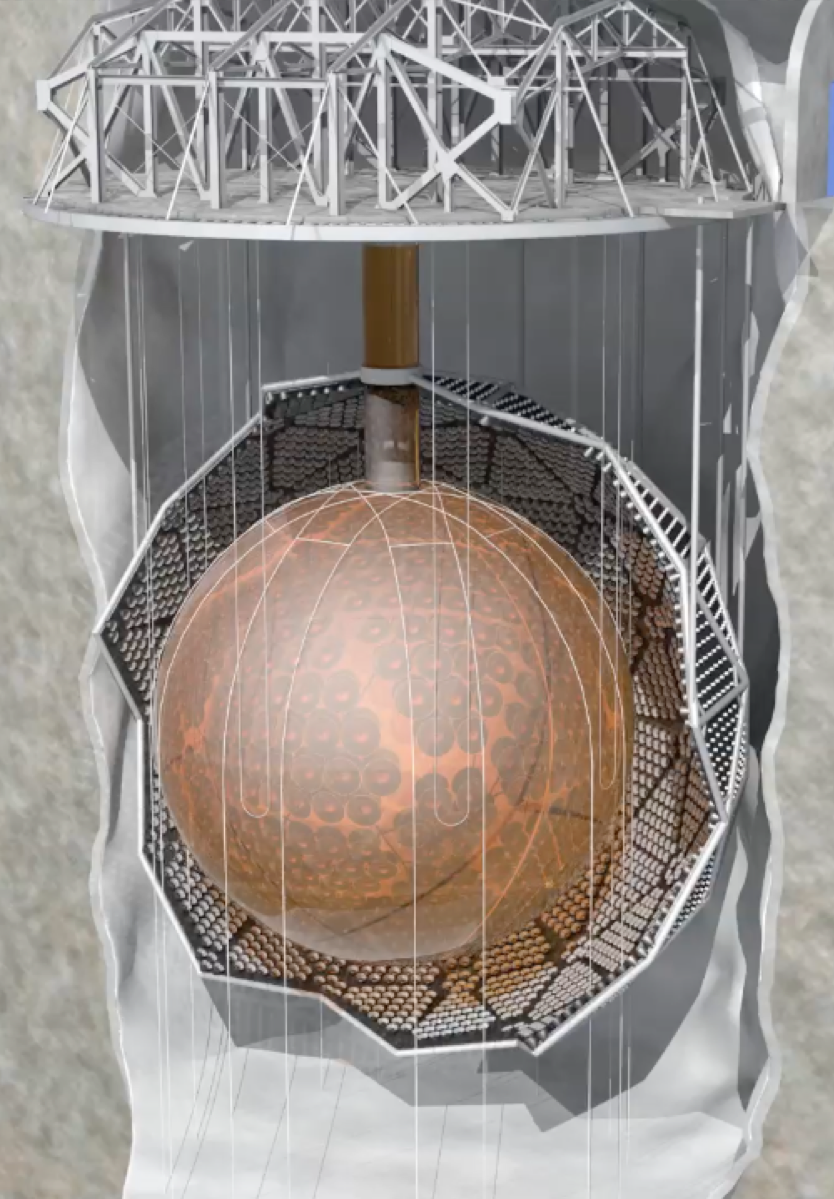
\includegraphics[width=0.7\textwidth]{images/detector_picture.png}
        \caption{Artistic impression of SNO+ detector~\cite{}}
        \label{fig:detector_pic}
    \end{subfigure}
    \begin{subfigure}{0.48\textwidth}
        \centering
        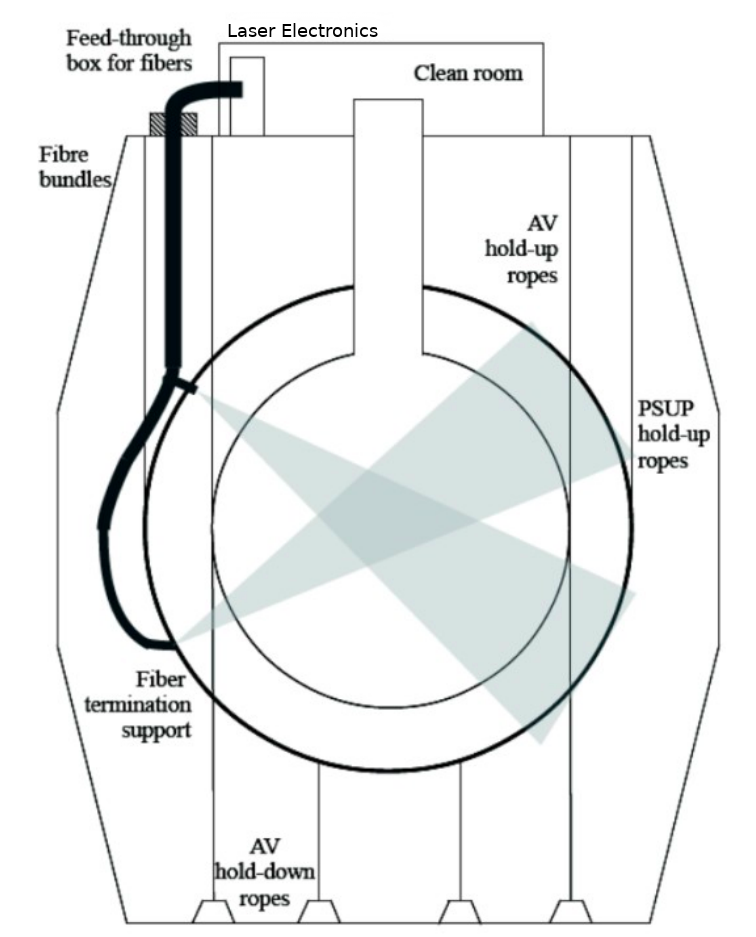
\includegraphics[width=0.8\textwidth]{images/SMELLIE_picture_corrected.png}
        \caption{Diagram of the SMELLIE calibration system, modified from~\cite{}.}
        \label{fig:smellie_diagram}
    \end{subfigure}
    \caption{Diagrams of the relevant geometries needed for this report.}
    \label{fig:diagrams}
\end{figure}